\documentclass[xetex]{beamer} % beamer = presentation type
\usepackage{fontspec}		% The XeTeX font spec package
\usepackage{xunicode}		% XeTeX Unicode character support
\usepackage{xltxtra}		% Umm something else XeTeX
\usepackage{url}

\usepackage{booktabs}	% Package for nicer tables

\usepackage{polyglossia}	% XeTeX multi-lingual support
\setmainlanguage{latvian}
\setotherlanguages{english,russian}

\newcommand{\termEn}[1]{\textenglish{\itshape {#1}}} % inline English

%\newfontfamily\japfont{IPAPMincho}
%\newfontfamily\japfont{IPAPGothic}
%\setmainfont{DejaVu Sans}
%\setsansfont{DejaVu Sans}
%\newfontfamily\IPA[Scale=MatchUppercase]{DejaVu Sans}


\author{Jānis Šmēdiņš}
\title[Mikrokontroliera kodola izstrāde]
	{Iekļautās sistēmas mikrokontroliera kodola izstrāde}
%\titlegraphic{\includegraphics[height=0.5\textheight]{img/Thistle.pdf}}
%\date{November 30, 2011}

%\usetheme{Dresden}	% My usual
\usetheme{Warsaw}	% Similar to Dresden

%\usecolortheme{whale}	% Usually same as default

%\usefonttheme{structuresmallcapsserif}	% Use small caps for titles etc.

%% English determined number suffixes
%\renewcommand{\th}{\textsuperscript{th} }
\newcommand{\st}{\textsuperscript{st} }
\newcommand{\rd}{\textsuperscript{rd} }
\newcommand{\nth}{\textsuperscript{th} }

% External common image library
\graphicspath{{/home/johnlm/Development/resources/tex_graphics_lib/}{img/}}

% symbol dump : “ ” —

\begin{document}
	% Slide 1 : Titlepage
	\begin{frame}
		%\centering\includegraphics[height=0.4\textheight]{Thistle}\\
		\titlepage 	% The default generated title slide
	\end{frame}
	
	\begin{frame}{Mērķis un uzdevumi}
		\textbf{Mērķis}: Izveidot procesoru izmantošanai par
			mikrokontroliera kodolu un izstrādāt paraugimplementāciju
			šādam mikrokontrolierim.\\[1em]
		\textbf{Uzdevumi}:
		\begin{itemize}\small
			\item Kodola un perifēro komponenšu saskarnes definēšana;
			\item Kodola izmantojamās instrukciju kopas definēšana;
			\item Kodola un tā apakškomponenšu aprakstīšana VHDL;
			\item Paraugimplementācijas definēšana un aprakstīšana VHDL;
			\item Paraugimplementācijas sintēze uz FPGA platformas.
		\end{itemize}
	\end{frame}
	
	\begin{frame}{Kas ir \ldots ?}
		\begin{columns}
		\column{0.49\textwidth}
			\textbf{Mikrokontrolieris}\\
			\small
			Paškomplektēta datorsistēma vienā mikroshēmā, kurā iekļauta:
			\begin{itemize}
				\item Procesora kodols;
				\item Operatīvā atmiņa;
				\item Patstāvīgā atmiņa;
				\item Programmējamas ievades/izvades pieslēgvietas;
				\item (Iespējamas) standarta komunikāciju saskarnes.
			\end{itemize}
			Mikrokontrolierus parasti izmanto dažādu iekļauto sistēmu
			vadībai un/vai datu apstrādei.
		\column{0.49\textwidth}
			\textbf{FPGA}\\
			\small
			Lietotāja pārrprogramējama mikroshēma, kurā var ieprogrammēt:
			\begin{itemize}
				\item Kombinacionālos loģikos elementus;
				\item Trigerus;
				\item Operatīvās un \textit{Flash} atmiņas
					(ja pieejamas);
				\item Dažādas augstākminēto elementu kombinācijas,
			\end{itemize}
			ar programmatūras rīkiem sintezējot HDL aprakstus.
		\end{columns}
	\end{frame}
	
	\begin{frame}{Paraugimplementācija (Rev.~03)}{Uzbūve}
		~ % FIX: To avoid putting graphic into frame title
		{\def\svgscale{0.85} \small \input{img/uC-sheem.pdf_tex}}
	\end{frame}
	
	\begin{frame}{Paraugimplementācija (Rev.~03)}{Uzbūve}
		~ % FIX: To avoid putting graphic into frame title
		{\def\svgscale{0.85} \small \input{img/uC-progress.pdf_tex}}
	\end{frame}
	
	\begin{frame}{Paraugimplementācija (Rev.~03)}{Kodols}
		\begin{columns}
		\column{0.15\textwidth}
			{\def\svgscale{0.85} \small \input{img/klucis-core.pdf_tex}}
		\column{0.84\textwidth}
			\begin{itemize}
				\item Fon Neimaņa arhitektūra.
				\item 16 bitu instrukcijas.
				\item Vienkāršota, minimāla instrukciju kopa, līdzīgi RISC
					principam.
				\item Datu apmaiņa ar perifērajām komponentēm notiek caur
					atmiņas saskarni.
				\item \textit{Load/Store} princips darbībā ar ,,atmiņu''.
				\item Praktiski pilnībā aprakstīts VHDL.
			\end{itemize}
		\end{columns}
	\end{frame}
	
	\begin{frame}{Paraugimplementācija (Rev.~03)}{Kodols}
		\begin{columns}
		\column{0.15\textwidth}
			{\def\svgscale{0.85} \small \input{img/klucis-core.pdf_tex}}
		\column{0.84\textwidth}
			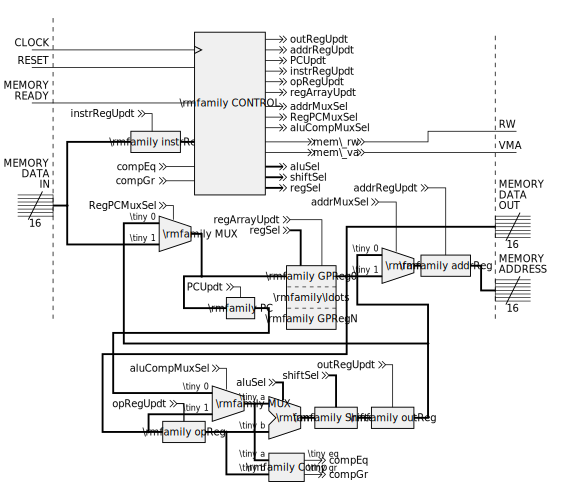
\includegraphics[width=0.9\textwidth]{top-rev3-detail.png}
		\end{columns}
	\end{frame}
	
	\begin{frame}{Paraugimplementācija (Rev.~03)}{Atmiņa}
		\begin{columns}
		\column{0.10\textwidth}
			{\def\svgscale{0.85} \small \input{img/rom-ram.pdf_tex}}
		\column{0.89\textwidth}
			\begin{itemize}
				\item Izmantoti \textit{Actel Fusion} pieejamie makrosi.
				\begin{itemize}%\small
					\item Lai izmantotu pieejamos \textit{Fusion} atmiņas resursus.
					\item Veiktspējas palielināšanai.
				\end{itemize}
				\item RAM apjoms: $16\mathrm{K} \times 16$
				\item ROM apjoms: $64 \times 16$
				\item RAM un ROM ir ar sinhronu darbību\\
					(Asinhronu darbību ,,emulē'' adrešu dekoderis).
			\end{itemize}
		\end{columns}
	\end{frame}
	
	\begin{frame}{Paraugimplementācija (Rev.~03)}{SPI saskarne}
		\begin{columns}
		\column{0.10\textwidth}
			{\def\svgscale{0.85} \small \input{img/klucis-spi.pdf_tex}}
		\column{0.89\textwidth}
			\begin{itemize}
				\item Realizē SPI \textit{Master} puses saskarni.
				\item Pilnībā aparatūras kontrolēta pārraide.
				\item Pārraida 16 bitu vai 8 bitu vārdu.
				\item Pārraides uzsākšana notiek ierakstot jaunus datus
					speciālā reģistrā.\\
					\texttt{\textcolor{blue}{ST} SPI\_PTR, Tx\_DATA}
				\item Saskarne pilnībā aprakstīta VHDL.
			\end{itemize}
		\end{columns}
	\end{frame}
	
	\begin{frame}{Darba progress}
		\textbf{Izdarītais}:
		\begin{itemize}\small
			\item Kodola komponenšu VHDL apraksti;
			\item Kodola augšējā līmeņa shēma;
			\item Kodola darbības simulācija;
			\item Adrešu dekodera VHDL apraksts;
			\item Kodola un Atmiņas komponenšu instancēšana mikrokontroliera
				augstākā līmeņa shēmā;
			\item Assembleris;
			\item \termEn{Boot} processa programma izpildprogrammas ielasei
				no SPI Flash.
		\end{itemize}
		\textbf{Darāmais}:
		\begin{itemize}\small
			\item GPIO saskarnes VHDL apraksts;
			\item Kopējās mikrokontroliera shēmas darbības pārbaudes;
			\item Fiziskā realizācija uz FPGA testa platformas.
		\end{itemize}
	\end{frame}
	
	\begin{frame}{Izmantotā literatūra}
		\begin{itemize} \small
			\item Michael J.~Flynn,\\
				\textit{Computer Architecture: Pipelined and Parallel Processor Design}\\
				London: Jones~and~Bartlett, 1995. ISBN~0-86720-204-1
			\item John von Neumann,
				\textit{First Draft of a Report on the EDVAC},\linebreak[2]
				University of Pennsylvania, 1945.
			\item Douglas L.~Perry,
				\textit{VHDL: Programming by Example}, 4\nth Edition. \linebreak[2]
				New York: McGraw-Hill, 2002. ISBN~0-07-140070-2
			\item Actel corp.,
				\textit{Fusion Embedded Development Kit User's Guide}, %\linebreak[2]
				%USA: Actel,
				2009.
			\item Actel corp.,
				\textit{Fusion FlashROM}, Application Note AC236, %\linebreak[2]
				%USA: Actel,
				2005.
			\item Actel corp.,
				\textit{Synplify — Synthesis Frequently Asked Questions}, %\linebreak[2]
				%USA: Actel,
				2009.
		\end{itemize}
	\end{frame}
	
	% Slide Last : Thank you!
	\begin{frame}
		\begin{center}
			\Large Paldies par uzmanību!\\[2em]
			%\normalsize It's now time for your questions.
		\end{center}
	\end{frame}
	
\end{document}

\begin{thebibliography}{9}
		\addcontentsline{toc}{section}{\refname}
		\bibitem{Flynn-arch}
			Michael J.~Flynn,
			\textit{Computer Architecture: Pipelined and Parallel Processor Design}
			\linebreak[3]
			London: Jones~and~Bartlett, 1995. ISBN~0-86720-204-1
		
		\bibitem{von-Neumann}
			John von Neumann,
			\textit{First Draft of a Report on the EDVAC},\linebreak[2]
			University of Pennsylvania, 1945.
		
		\bibitem{Perry-VHDL}
			Douglas L.~Perry,
			\textit{VHDL: Programming by Example}, 4\nth Edition. \linebreak[2]
			New York: McGraw-Hill, 2002. ISBN~0-07-140070-2
		
		\bibitem{FusionGuide}
			Actel corp.,
			\textit{Fusion Embedded Development Kit User's Guide}, %\linebreak[2]
			%USA: Actel,
			2009.
		
		\bibitem{FlashROM}
			Actel corp.,
			\textit{Fusion FlashROM}, Application Note AC236, %\linebreak[2]
			%USA: Actel,
			2005.
		
		\bibitem{FusionFAQ}
			Actel corp.,
			\textit{Synplify — Synthesis Frequently Asked Questions}, %\linebreak[2]
			%USA: Actel,
			2009.
